\section{Placement Results}
\label{sec:results}

Here, we present test results for a basic SA placer as well as test results for four simple variations as listed below. 
Note that midpoint simply means centroid.

\begin{itemize}
    \item \texttt{PlacerGreedyRandom}: all undirected random moves with greedy acceptance
    \item \texttt{PlacerGreedyMidpoint}: all directed centroid moves with greedy acceptance
    \item \texttt{PlacerAnnealRandom}: all undirected random moves with annealing acceptance \textbf{(the basic SA algorithm)}
    \item \texttt{PlacerAnnealMidpoint}: all directed centroid moves with annealing acceptance
    \item \texttt{PlacerAnnealHybrid}: 50\% random - 50\% centroid moves with annealing acceptance
\end{itemize}

{
    \centering
    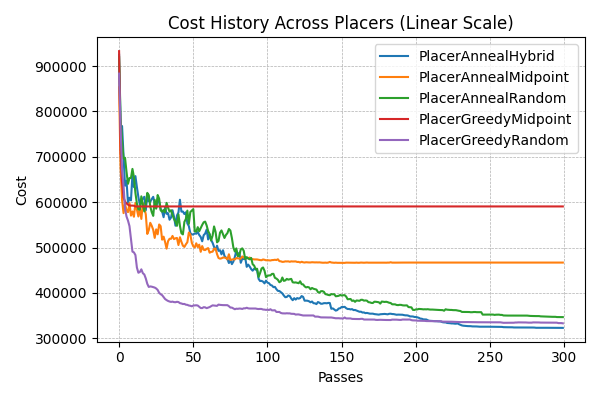
\includegraphics[width=\columnwidth]{figures/results/combined_cost_history_linear.png}
    \captionof{figure}{All placers overlaid}
    \label{fig:placers_overlay}
}

\newcolumn
{
    \centering
    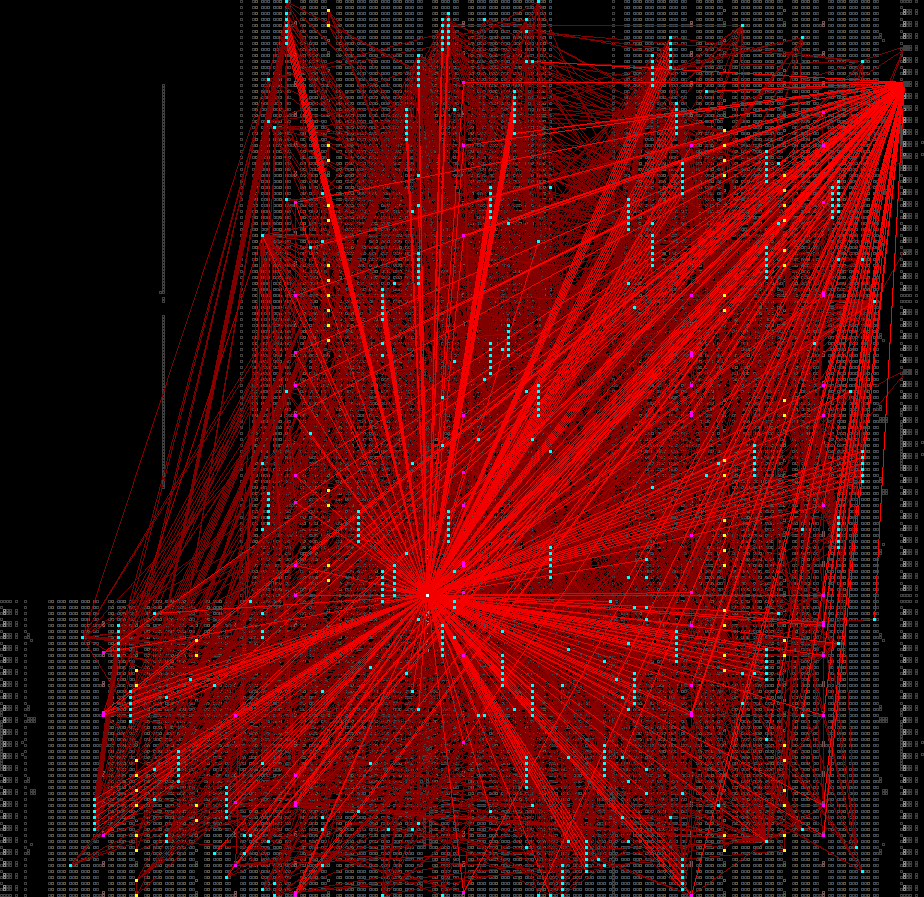
\includegraphics[valign=t, scale=0.13]{figures/results/PlacerGreedyRandom/random_placement.png}
    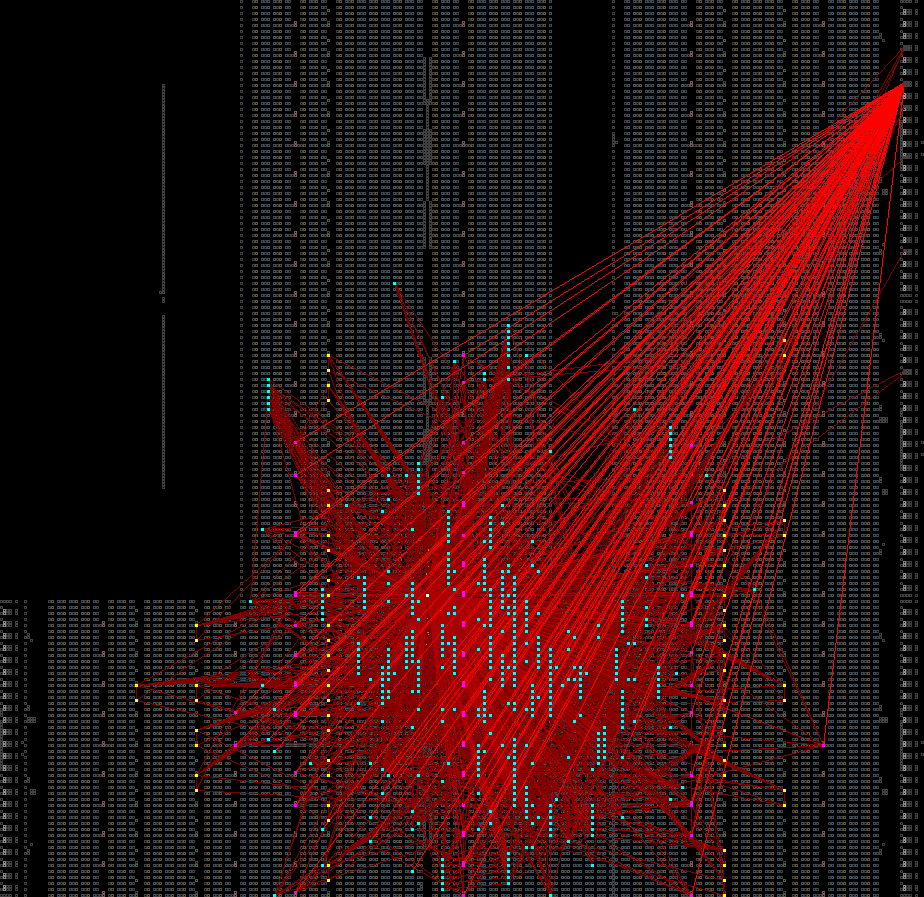
\includegraphics[valign=t, scale=0.13]{figures/results/PlacerGreedyRandom/00000010.png}
    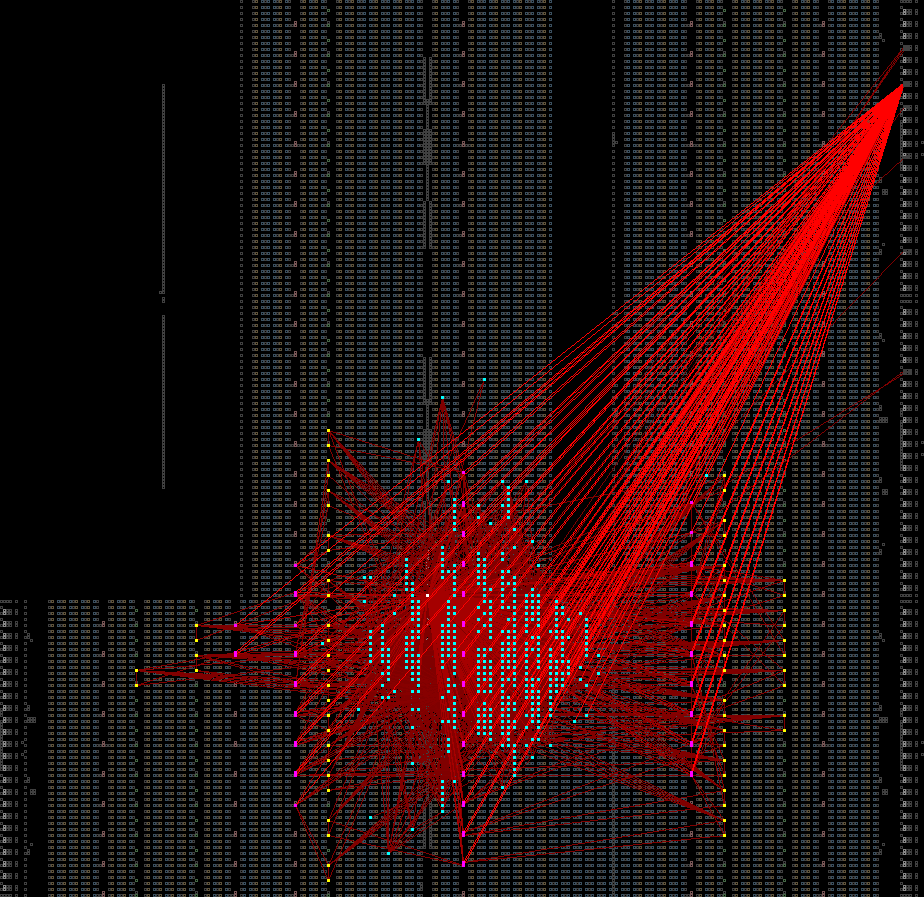
\includegraphics[valign=t, scale=0.13]{figures/results/PlacerGreedyRandom/00000100.png}
    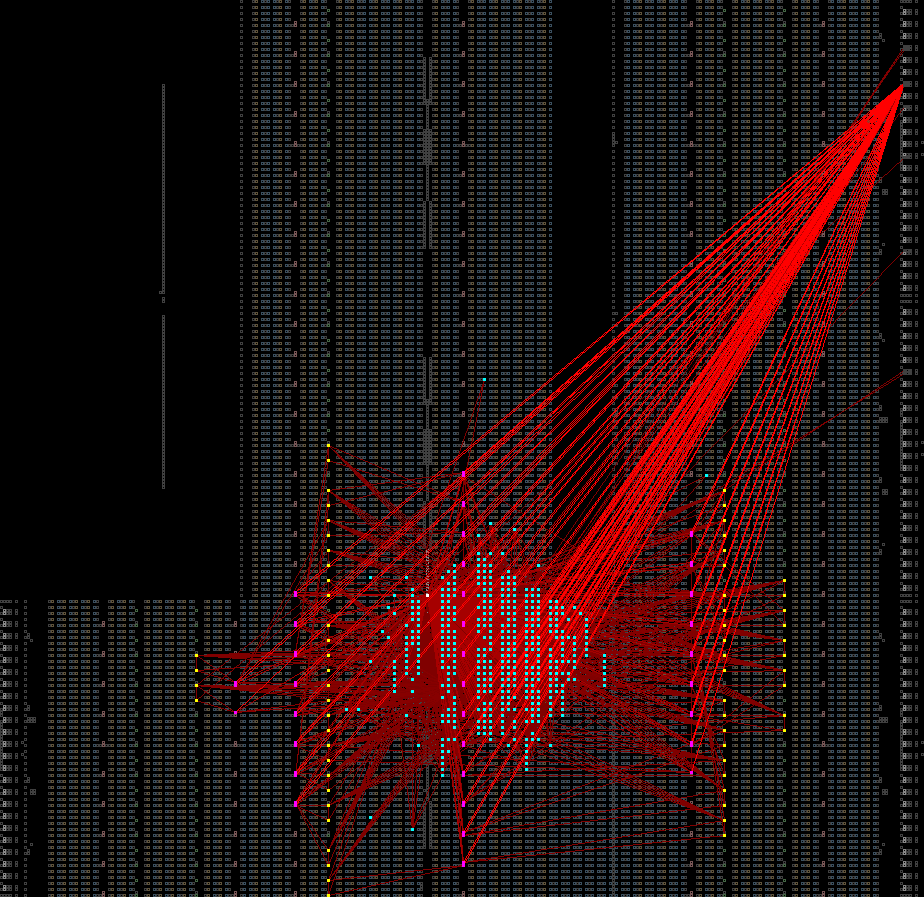
\includegraphics[valign=t, scale=0.13]{figures/results/PlacerGreedyRandom/00000299.png}
    \captionof{figure}{PlacerGreedyRandom}
    \label{fig:PGRSnapshots}
}

\newcolumn
{
    \centering
    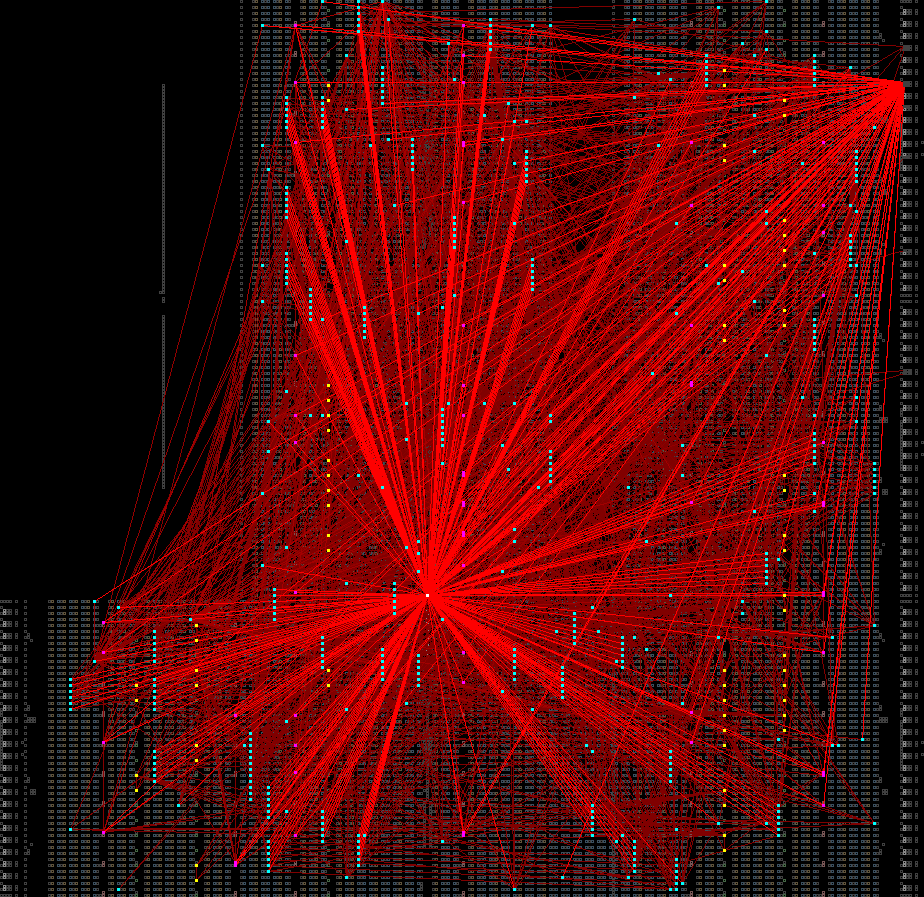
\includegraphics[valign=t, scale=0.13]{figures/results/PlacerGreedyMidpoint/random_placement.png}
    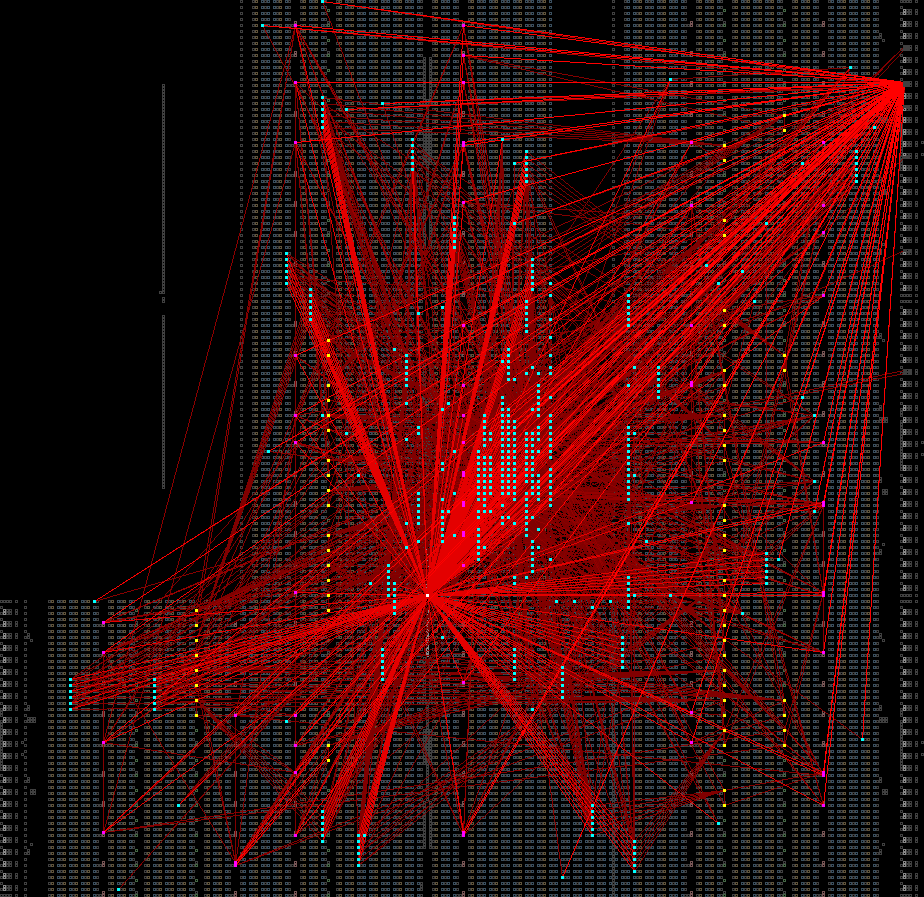
\includegraphics[valign=t, scale=0.13]{figures/results/PlacerGreedyMidpoint/00000010.png}
    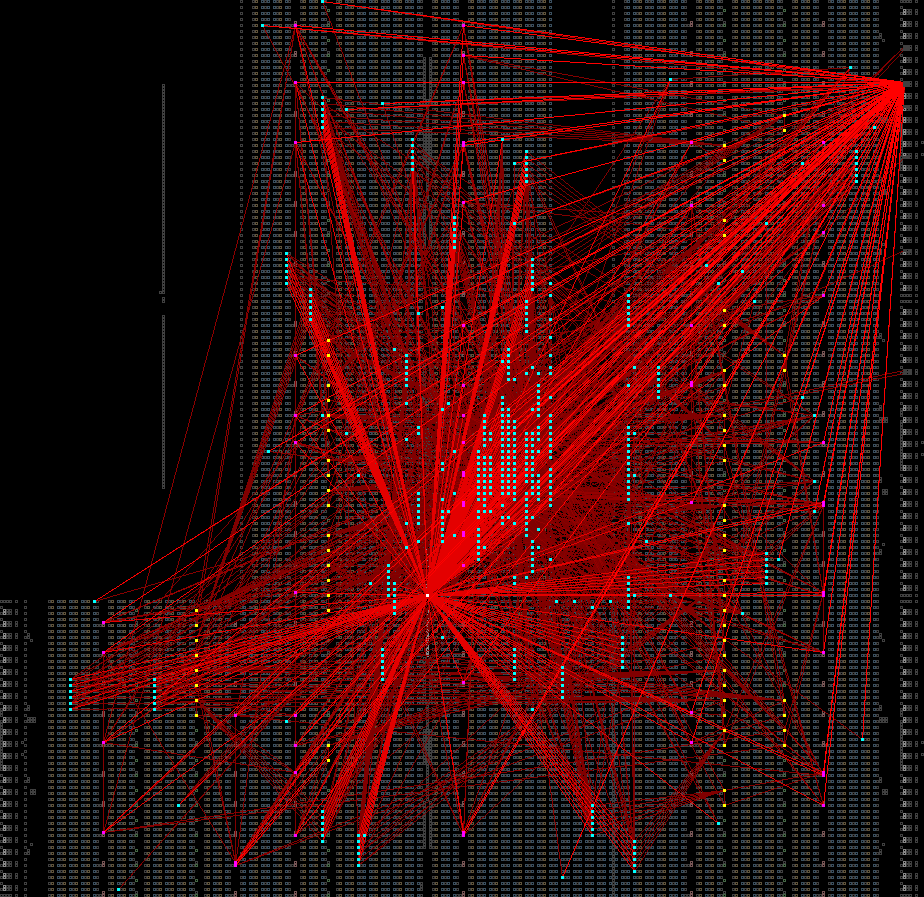
\includegraphics[valign=t, scale=0.13]{figures/results/PlacerGreedyMidpoint/00000100.png}
    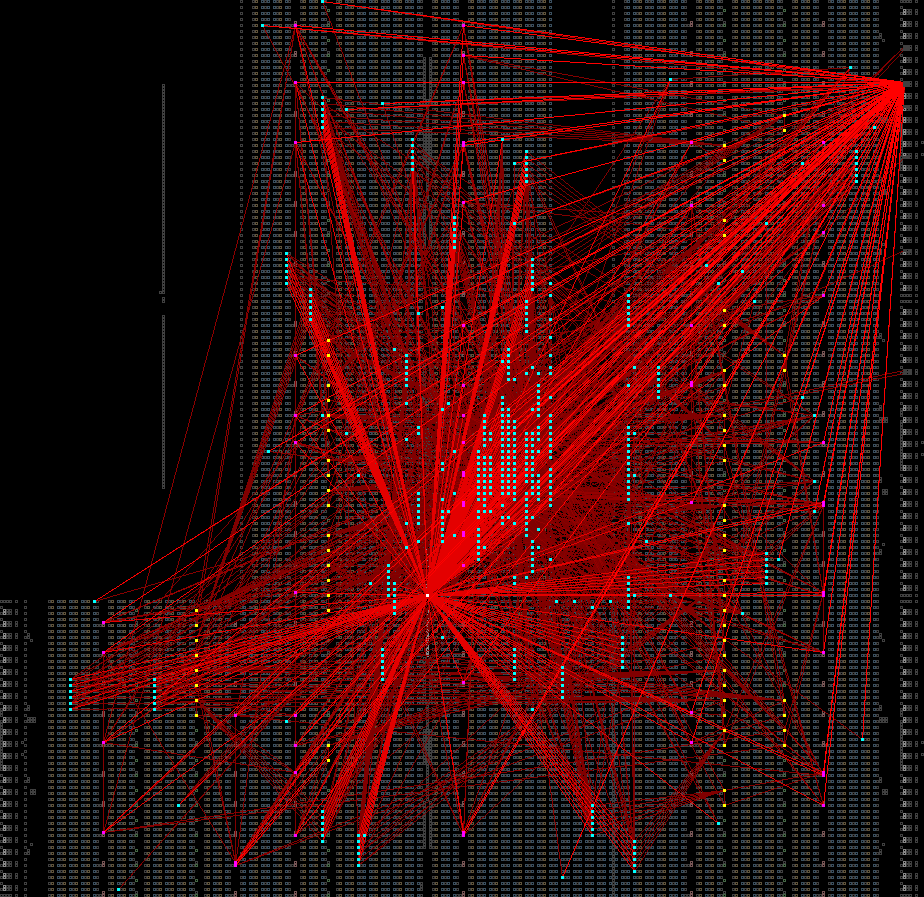
\includegraphics[valign=t, scale=0.13]{figures/results/PlacerGreedyMidpoint/00000299.png}
    \captionof{figure}{PlacerGreedyMidpoint}
    \label{fig:PGMSnapshots}
}

{
    \centering
    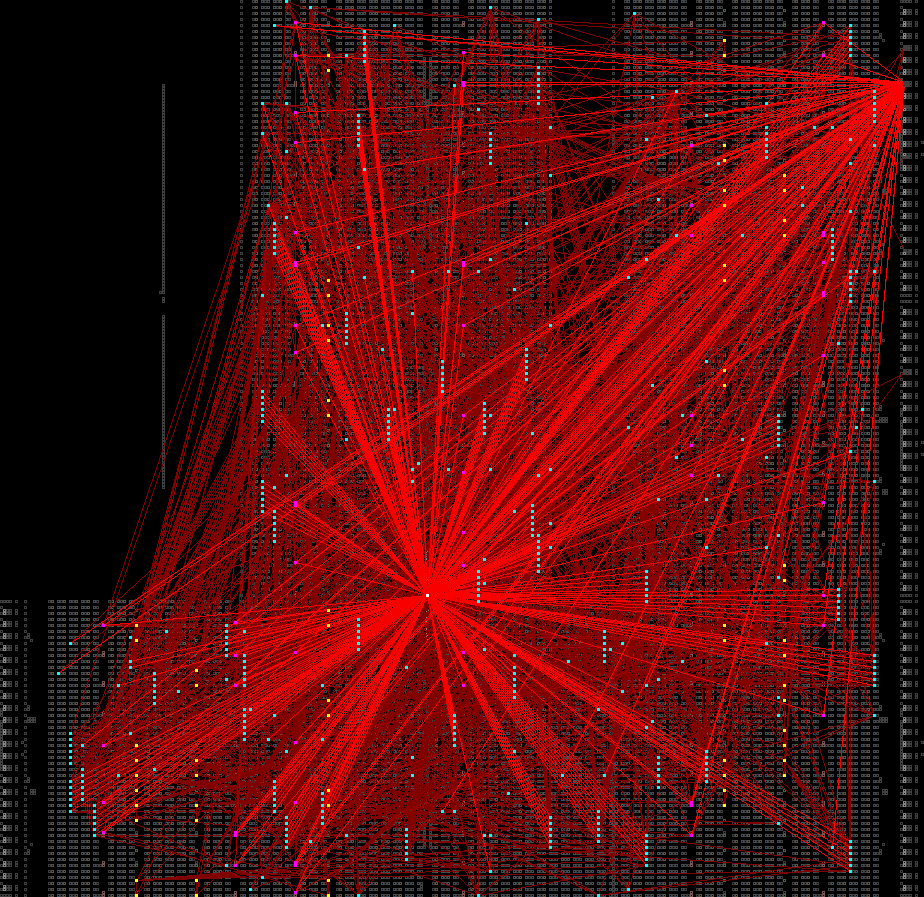
\includegraphics[valign=t, scale=0.13]{figures/results/PlacerAnnealRandom/random_placement.png}
    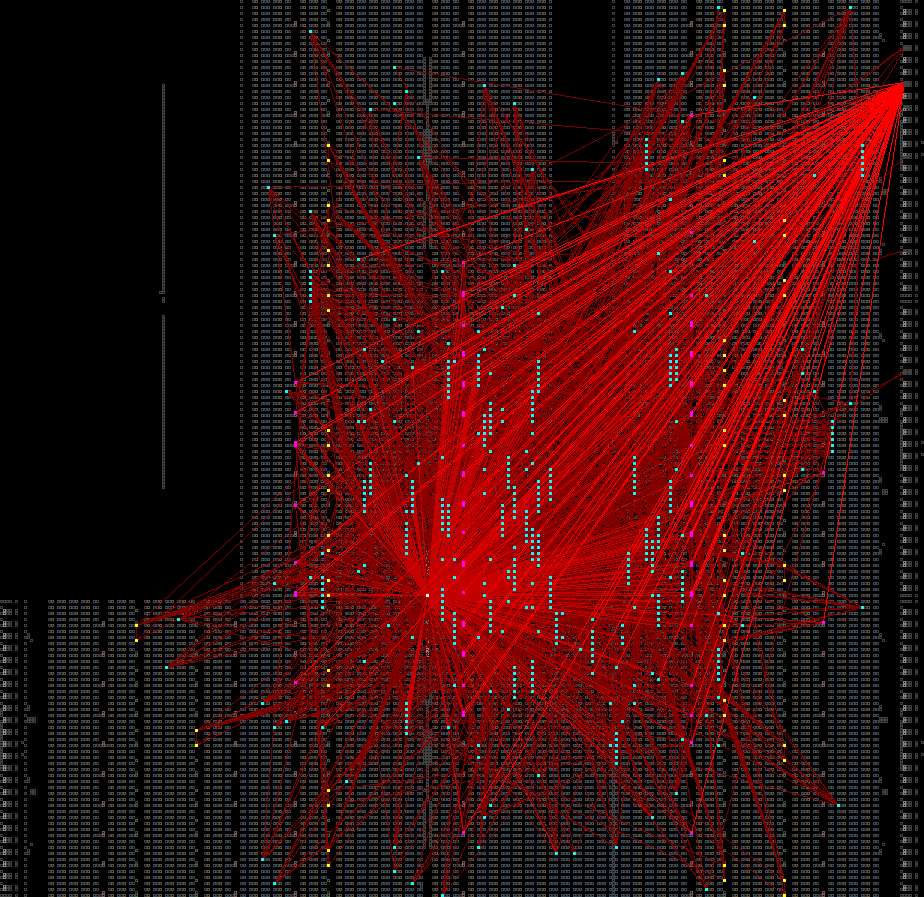
\includegraphics[valign=t, scale=0.13]{figures/results/PlacerAnnealRandom/00000010.png}
    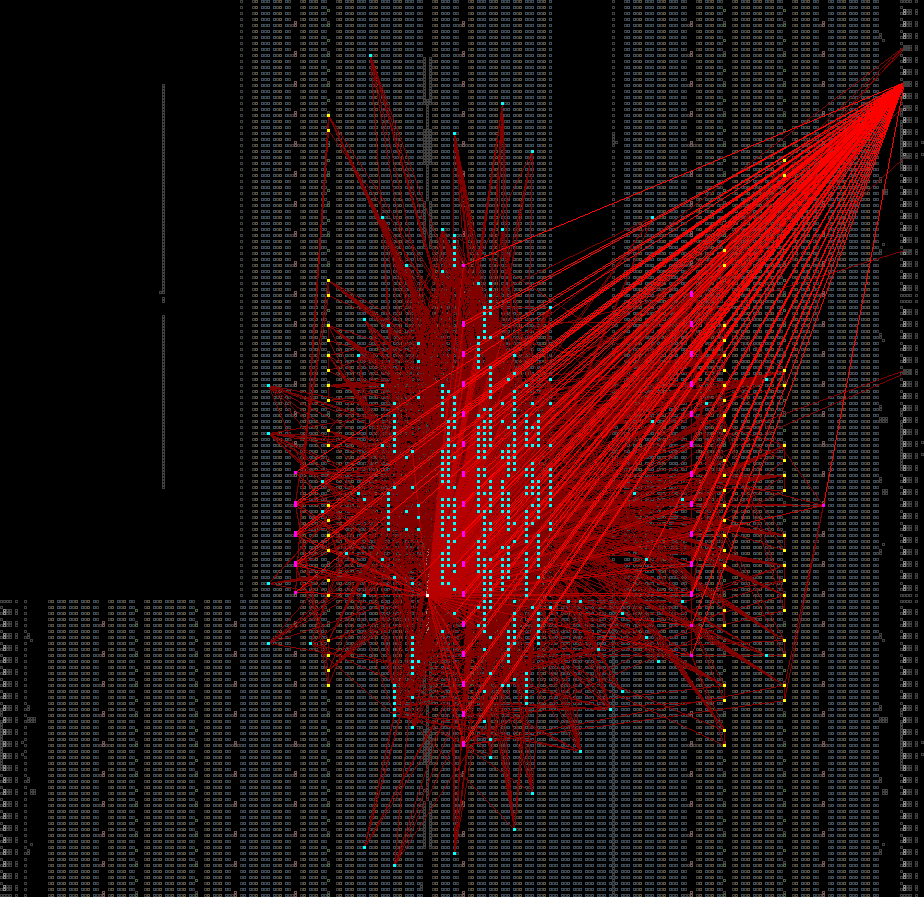
\includegraphics[valign=t, scale=0.13]{figures/results/PlacerAnnealRandom/00000100.png}
    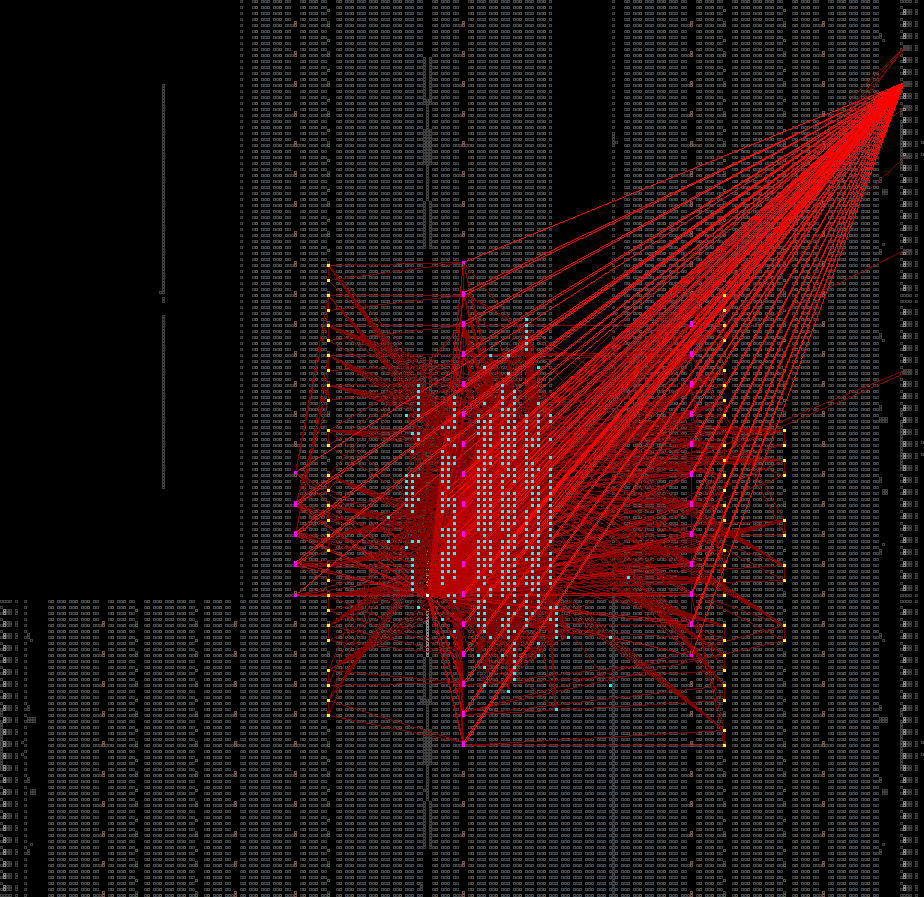
\includegraphics[valign=t, scale=0.13]{figures/results/PlacerAnnealRandom/00000299.png}
    \captionof{figure}{PlacerAnnealRandom}
    \label{fig:PARSnapshots}
}

\newcolumn
{
    \centering
    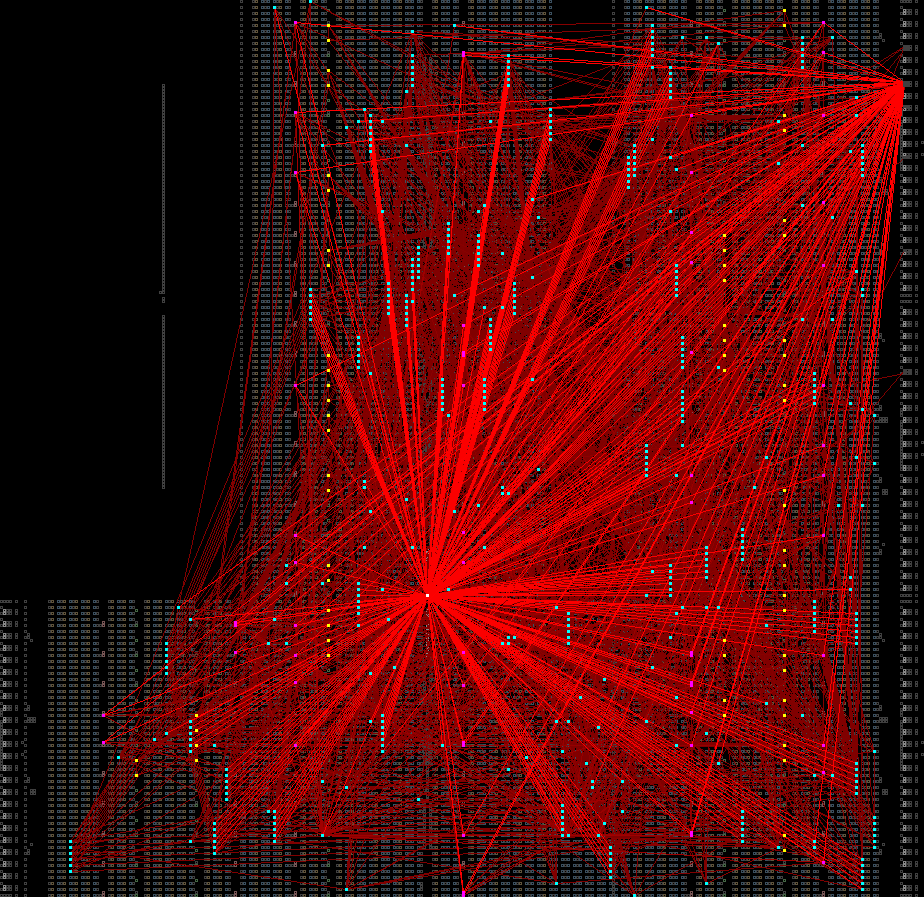
\includegraphics[valign=t, scale=0.13]{figures/results/PlacerAnnealMidpoint/random_placement.png}
    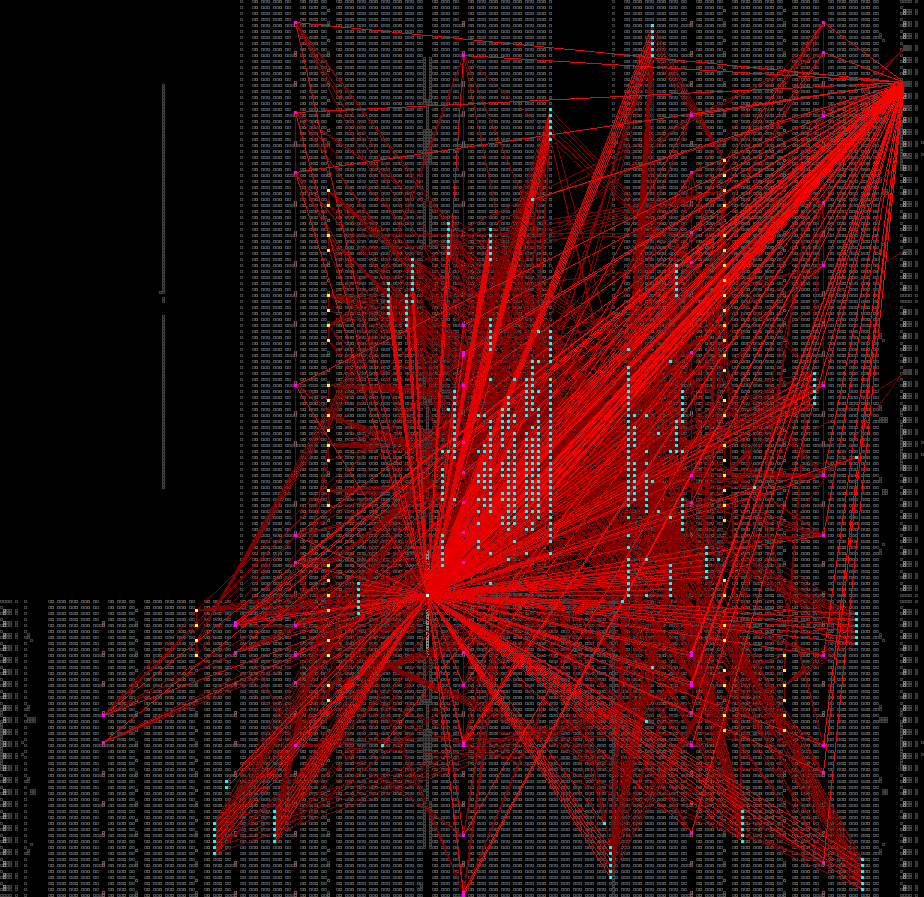
\includegraphics[valign=t, scale=0.13]{figures/results/PlacerAnnealMidpoint/00000010.png}
    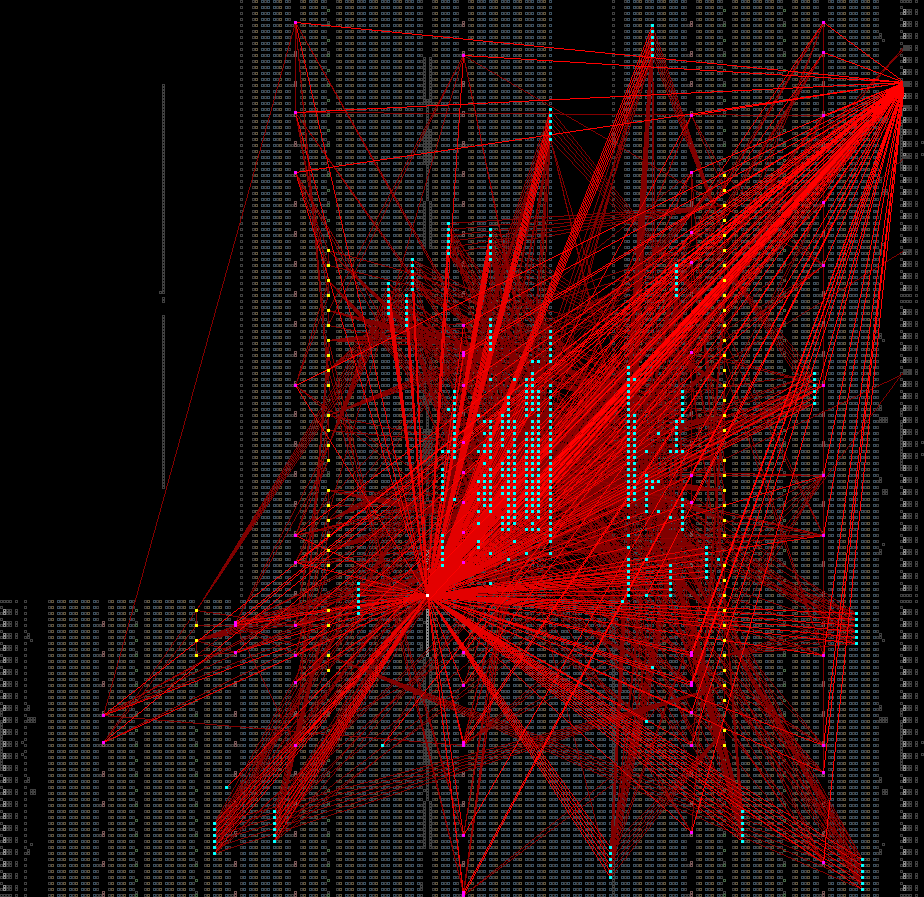
\includegraphics[valign=t, scale=0.13]{figures/results/PlacerAnnealMidpoint/00000100.png}
    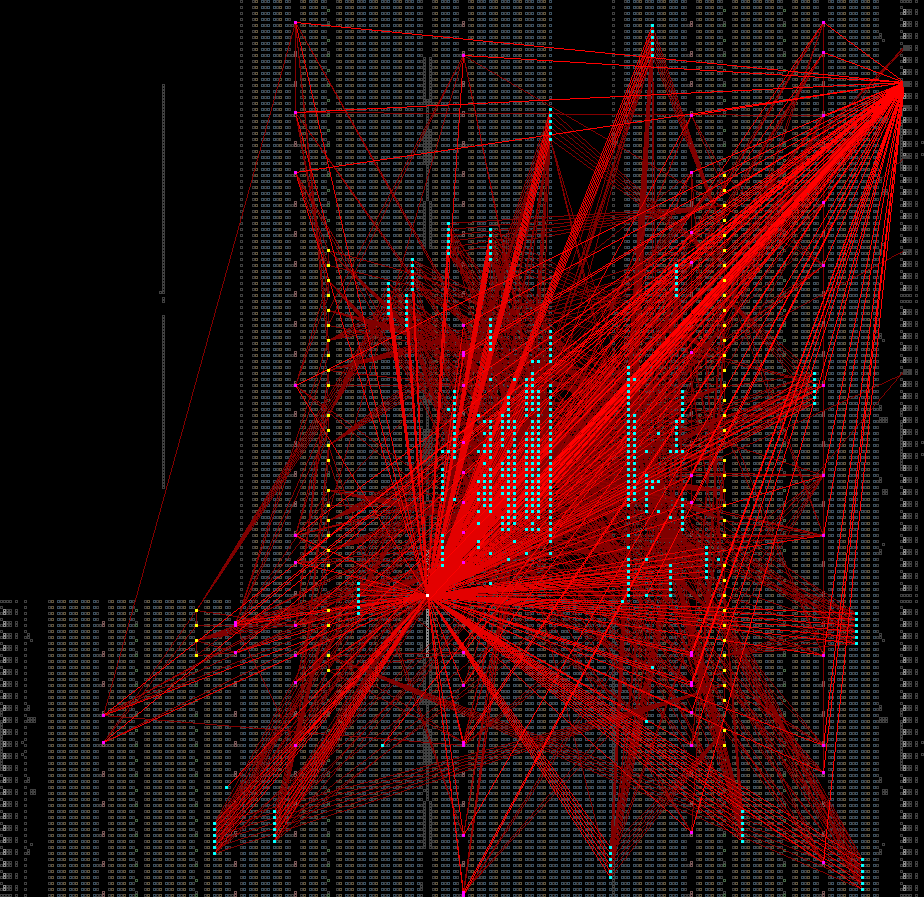
\includegraphics[valign=t, scale=0.13]{figures/results/PlacerAnnealMidpoint/00000299.png}
    \captionof{figure}{PlacerAnnealMidpoint}
    \label{fig:PAMSnapshots}
}

{
    \centering
    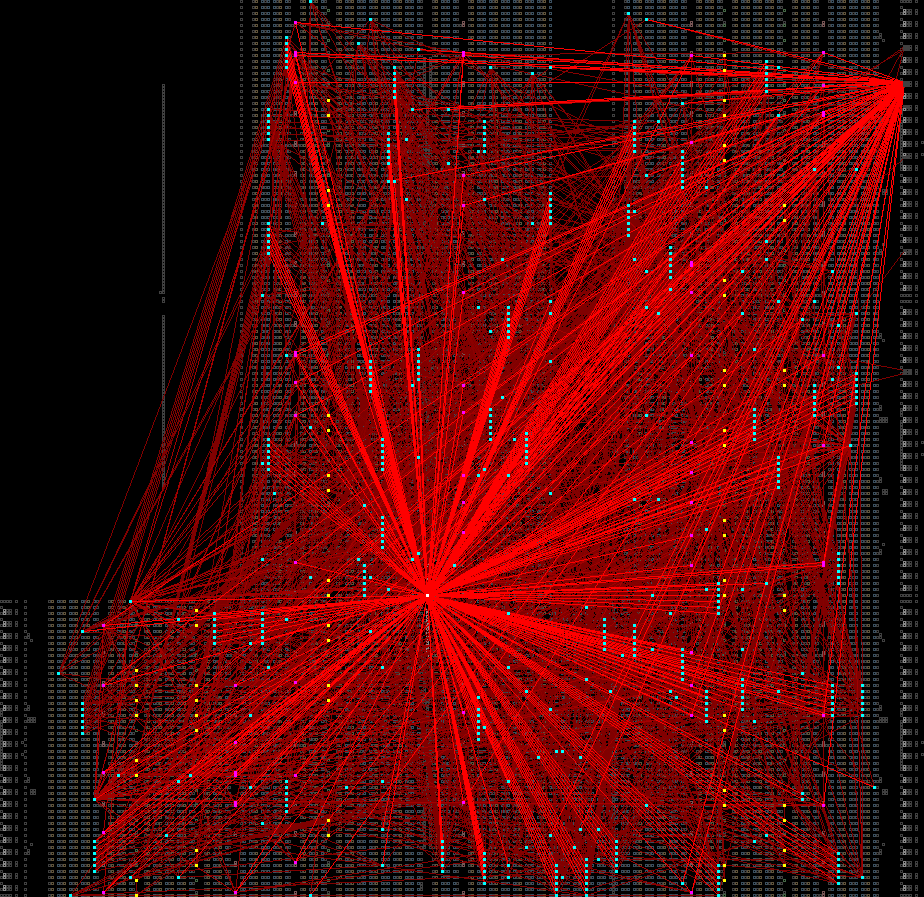
\includegraphics[valign=t, scale=0.13]{figures/results/PlacerAnnealHybrid/random_placement.png}
    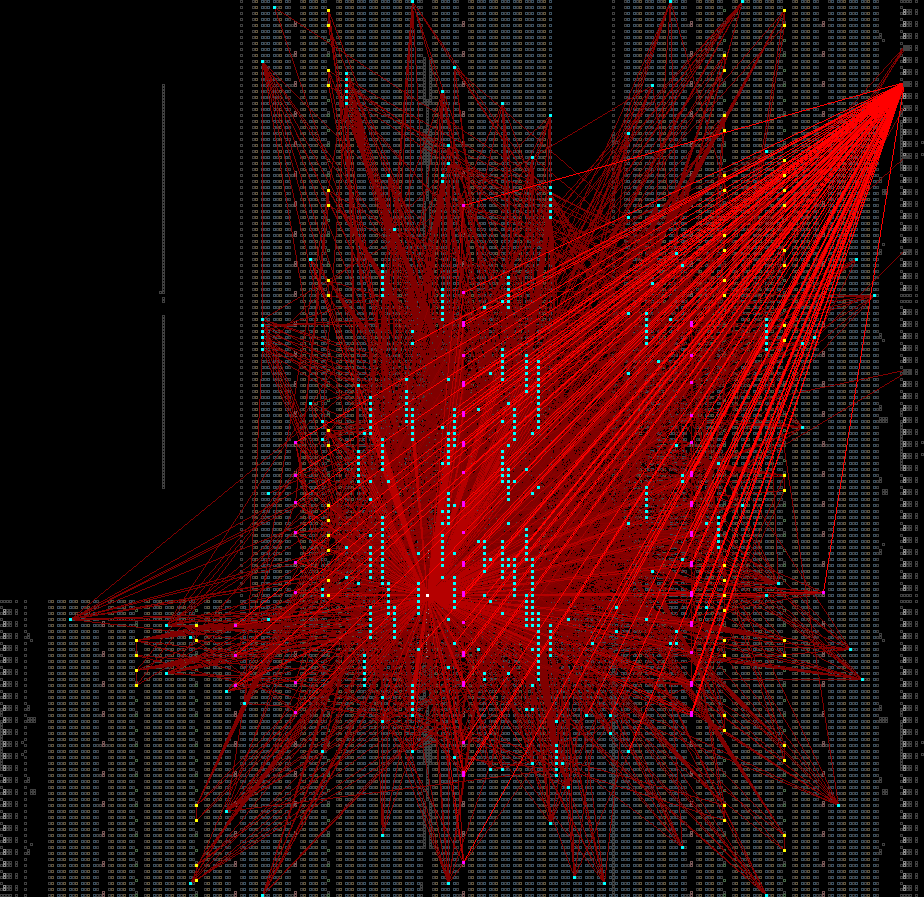
\includegraphics[valign=t, scale=0.13]{figures/results/PlacerAnnealHybrid/00000010.png}
    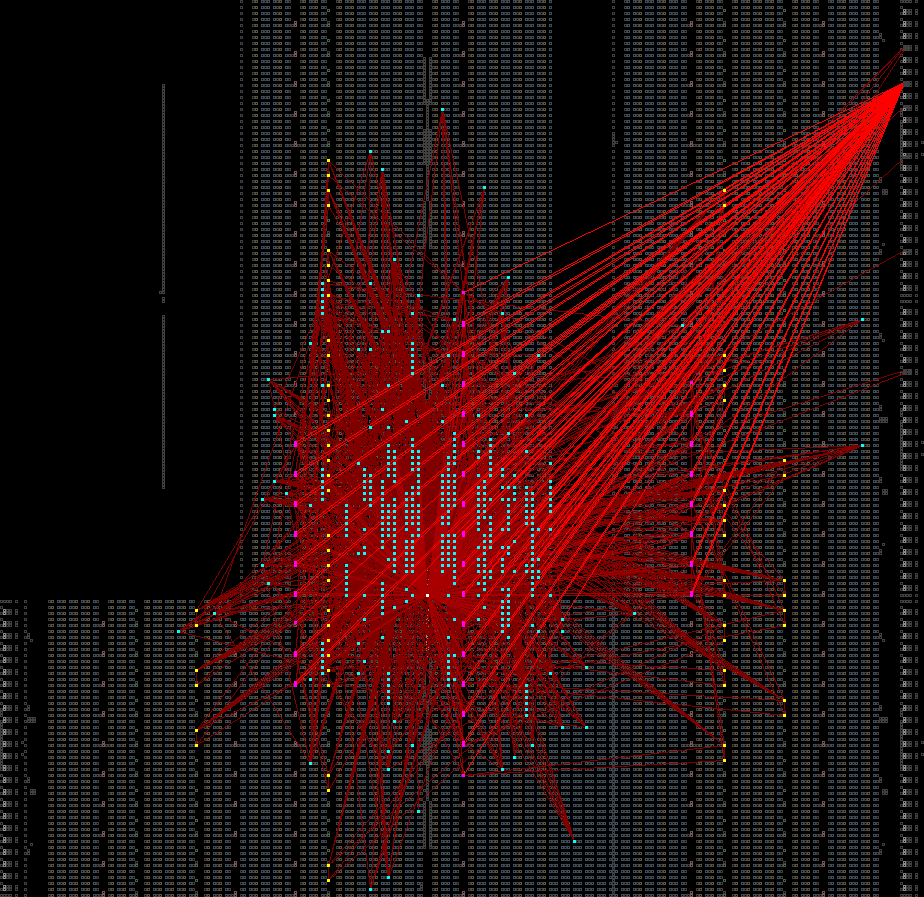
\includegraphics[valign=t, scale=0.13]{figures/results/PlacerAnnealHybrid/00000100.png}
    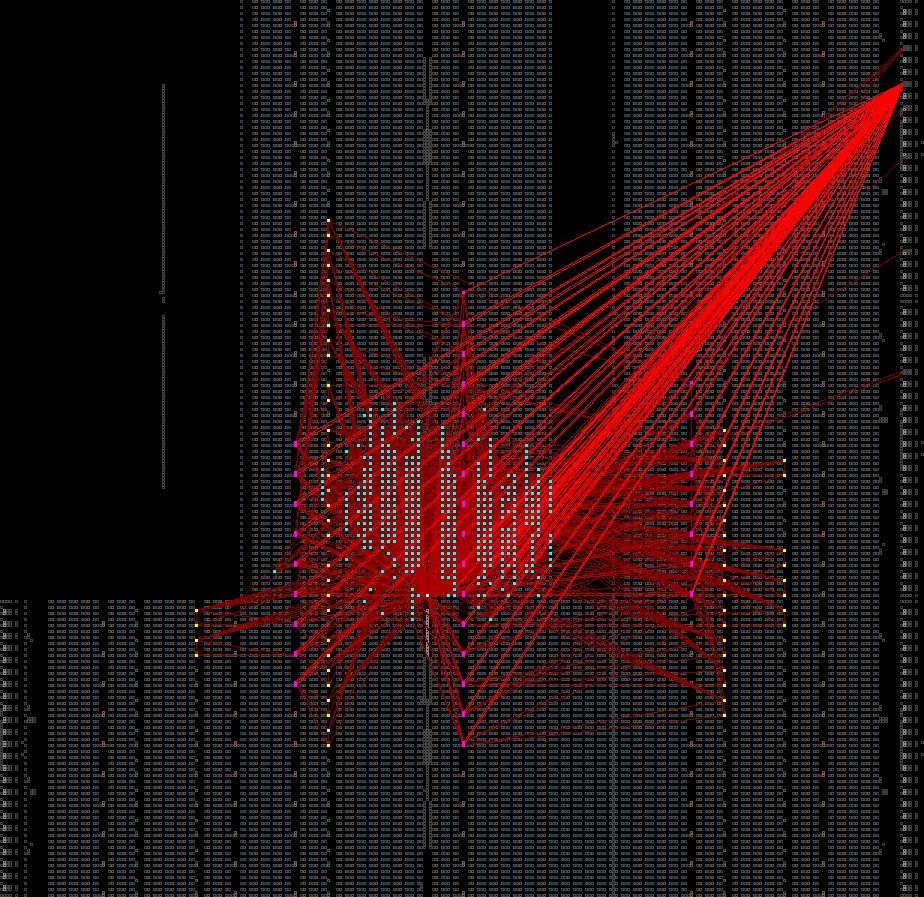
\includegraphics[valign=t, scale=0.13]{figures/results/PlacerAnnealHybrid/00000299.png}
    \captionof{figure}{PlacerAnnealHybrid}
    \label{fig:PAHSnapshots}
}
% {
%     \centering
%     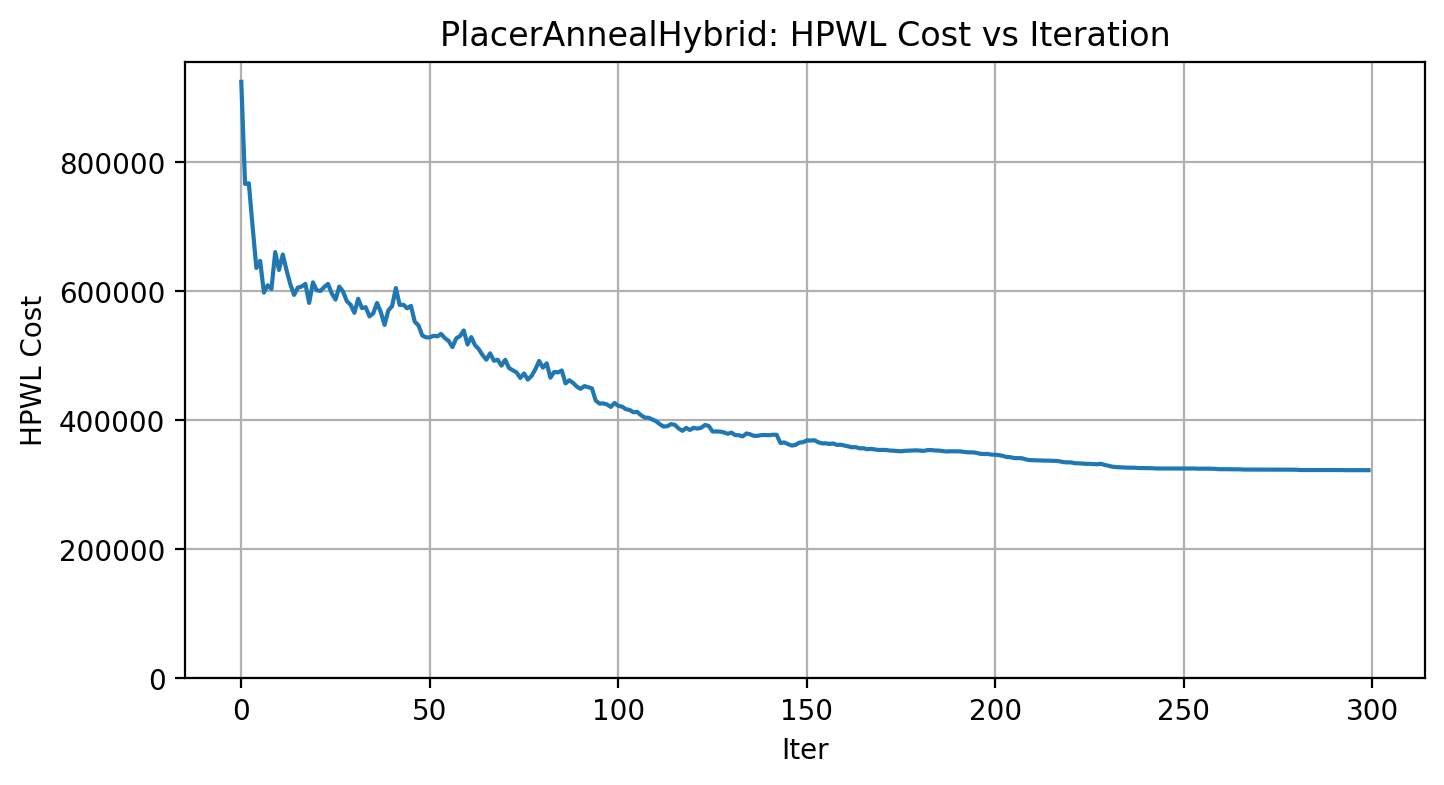
\includegraphics[width=0.7\columnwidth]{figures/results/PlacerAnnealHybrid/PlacerAnnealHybrid_cost_history.png}
%     \captionof{figure}{Total HPWL Cost vs number of passes. Final cost: 322933.}
%     \label{fig:PAHCurve}
% }



\begin{multicols}{2}
